\documentclass[12pt]{article}
\usepackage[margin=1in]{geometry} 
\usepackage{amsmath,amsthm,amssymb,amsfonts}
\usepackage{graphicx}
\usepackage{placeins}
\usepackage{listings} % Required for insertion of code
\usepackage[normalem]{ulem} % for underline
\usepackage{caption}
\usepackage{subcaption}
\usepackage{float}


\newcommand{\N}{\mathbb{N}}
\newcommand{\Z}{\mathbb{Z}}
\renewcommand{\lstlistingname}{Code}

\lstset{language=C,frame=single,breaklines=true,showstringspaces=false}
 
\newenvironment{problem}[2][Problem]{\begin{trivlist}
\item[\hskip \labelsep {\bfseries #1}\hskip \labelsep {\bfseries #2.}]}{\end{trivlist}}
%If you want to title your bold things something different just make another thing exactly like this but replace "problem" with the name of the thing you want, like theorem or lemma or whatever
 
\begin{document}
 
%\renewcommand{\qedsymbol}{\filledbox}
%Good resources for looking up how to do stuff:
%Binary operators: http://www.access2science.com/latex/Binary.html
%General help: http://en.wikibooks.org/wiki/LaTeX/Mathematics
%Or just google stuff
 
\title{\textbf{Fast Iterative Solvers: \\Project 2}}

\author{Jaeyong Jung (359804)}
\maketitle

\newpage


\FloatBarrier

\textbf{1. Plot the convergence using the measure $||r^{m} ||_{\infty} /||r^{0}||_{\infty}$ against multigrid iterations m for meshes with n = 4, n = 7 (resulting in N = 16, and N = 128).}
\\

To begin with, $n=4$ is tried to see the convergence. Simulation is done for two cases by varying $\nu$ as described in Figure 1. The maximum number of iteration is 30.


\begin{figure}[H]
\centering
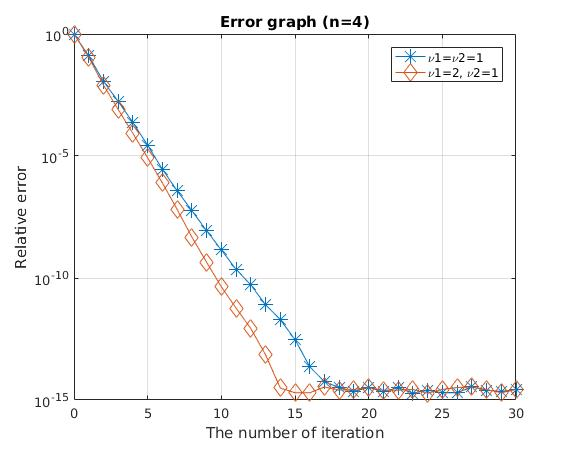
\includegraphics[scale=0.7]{err.jpg}
\caption{Error analysis when n is 4}
\end{figure}

For the first case, $\nu1=\nu2=1$, The relative error decreases drastically until \textbf{18-th} iteration step. At that \textbf{18-th} point, the relative error is $3.239\times10^{-15}$. Then it reaches $2.699\times10^{-15}$ at last. On the other hand, the later case, $\nu1=2, \nu2=1$, convergency is attained much faster. Untill \textbf{15-th} iteration, the relative error diminishes rapidly. At that point, relative error is $1.979\times10^{-15}$, which is even less than the first case's error at \textbf{18-th} point. Finally, the error at \textbf{30-th} step is $2.699\times10^{-15}$ and it is identical to that of the first case. Two cases' final value is the same. Nevertheless, the second case shows oscilating behavior. At the \textbf{15-th} the error is $1.979\times10^{-15}$ but the last error is bigger, $2.699\times10^{-15}$. It is guessed that coarsness of the mesh yield the oscillating bahavior. By comparing this result with numerical simulation with finer mesh, this guess will be verified.   

Computational experiment with $n=7$ is done to see if the rate of convergence is higher compared to coarser mesh. The result is shown on Figure 2.

\begin{figure}[H]
\centering
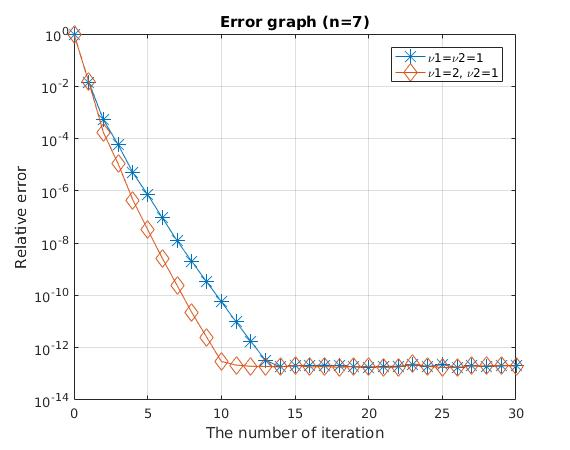
\includegraphics[scale=0.7]{err7.jpg}
\caption{Error analysis when n is 7}
\end{figure}

When $\nu1=\nu2=1$, the relative error decreases drastically until \textbf{13-th} iteration step. At that \textbf{13-th} point, the relative error is $3.288\times10^{-13}$. Then it reaches $2.109\times10^{-13}$ at last, \textbf{30-th} step. On the other hand, the later case, $\nu1=2, \nu2=1$, convergency is attained much faster. Untill \textbf{10-th} iteration, the relative error diminishes rapidly. At that point, relative error is $2.976\times10^{-13}$, which is even less than the first case's error at \textbf{13-th} point. Finally, the error at \textbf{30-th} step is $1.951\times10^{-13}$ and it is smaller as well.  

In summary, it takes less iteration step for finer mesh to get convergence. Plus, finer mesh does hot have oscillating behavior. For both of them, more Gauss-Seidel pre-smoothing step makes numerical solution to converge with less iterations. However, the final iteration's value of error is smaller in coarser mesh. That is because the size of mesh is closer to the lowest level, where the equation is perfectly solved, for coarser mesh. 
\\



%\begin{figure*}[h]
%    \centering
%    \begin{subfigure}[h]{0.5\textwidth}
%        \centering
%        \includegraphics[height=1.2in]{coarse_interpolation.jpeg}
%        \caption{coarse mesh}
%    \end{subfigure}%
%    ~ 
%    \begin{subfigure}[h]{0.5\textwidth}
%        \centering
%        \includegraphics[height=1.2in]{fine_interpolation.jpeg}
%        \caption{fine mesh}
%    \end{subfigure}
%    \caption{Comparing graph of coarse and fine mesh}
%\end{figure*}



\textbf{2. Further consideration about the effect of pre-Gauss-Seidel smoothing operation.)}
\\

The comparision of numerical experiments showed that pre-Gauss-Seidel smoothing will make the multigrid process to require less iteration for convergence. Nevertheless, it does not necessarily mean that more smoothing will take less time for convergence as well. Thus, it is necessary to conduct numerical experiment to compare runtimes. Before the comparision is done, other parameters are defined. $n=7$ and $\nu2=1$. $\nu1$ is changed every time to see difference in runtime.

\begin{figure}[H]
\centering
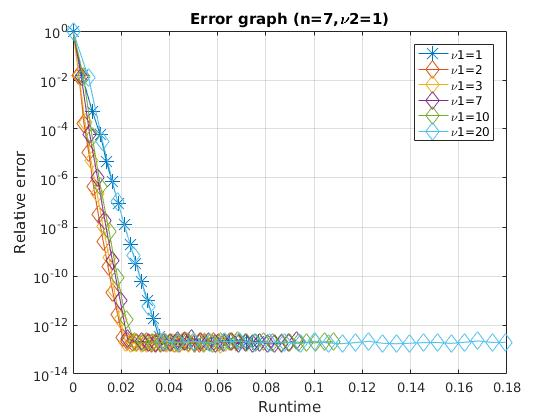
\includegraphics[scale=0.7]{runtime.jpg}
\caption{Runtime comparision}
\end{figure}

The convergence criteria is the point that relative error goes below $10^{-12}$. 

The fastest convergence in error is made when $\nu1=2$ and it takes $20.63ms$. The slowest case is when $\nu1=20$, and the runtime is $37.62ms$. The graph in Figure 3 proves that there is optimal number of smoothing. If there is too much smoothing, it will not only decrease the performance of computation but also takes more time than one smoothing. In conclusion, two or three times for smoothing is optimal. 
\\

\textbf{3. Implementations of Gauss-Seidel Smoother, restriction operator, prolongation, and main function.}
\\
Important functions are copied on following page. The entire code is also submitted.
\\

C code:
\lstinputlisting[language=C]{codes.c}






\end{document}


